%!TEX root = ../main.tex

In this chapter we discuss how the Transactions, introduced in 
Chapter~\ref{ch:transactions} are included in a block in the hash-chain,
introduced in Chapter~\ref{ch:hashchain}.

In Chapter~\ref{ch:transactions} we said that all transactions are broadcast, validated and applied by every node. However applying transactions in different order may cause the system to diverge.

\section{Centralized straw-man system}
We present a straw man solution that relies on a centralized leader to include transactions into a block and issue those blocks. 
After discussing difficulties with this approach, we present the proof of work based scheme used in bitcoin.

As shown in Figure~\ref{fig:leader}, 
We assume a single leader exists. Transactions are submitted to the leader.
At regular intervals, the leader includes all new (and valid) transactions in a merkle tree. The root of the merkle-tree is included in a new block.

The block is then broadcast to all participating nodes, who validate it.
\emph{The validation of blocks prevents the leader from including malformed transactions}. 
However this system still opens several ways for the leader to misbehave:
\begin{enumerate}[label=\Alph*)]
	\item The leader can omit certain transactions on purpose. (Censorship)
	\item The leader is a single point of failure.
	\item The leader could send different blocks to different processes.
\end{enumerate}
\comment{If bitcoin would have a leader, some agency would have shut it down long ago.}



\begin{figure}
	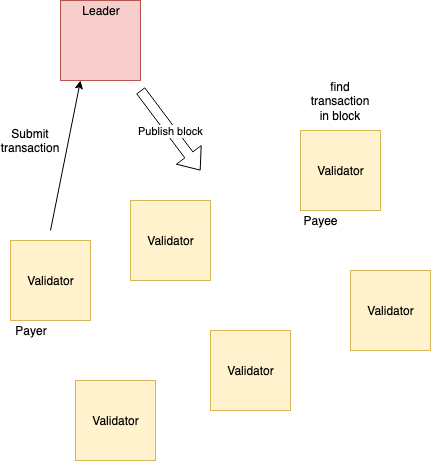
\includegraphics{fig/Leader}
	\caption{Straw-man system with leader. Payer submits transaction to the leader. The payee will eventually find the transaction in a block and know he was payed.}
	\label{fig:leader}
\end{figure}

\pagebreak
\section{PoW function}
Before we can discuss, how bitcoin avoids a single leader, we have to learn about PoW functions.

\begin{definition}\label{def:pow1}
	(PoW function version 1)
	For an integer $d$,
	the proof-of-work (PoW) function with difficulty $d$ takes a data item and returns a nonce (random bits) and a hash value:
	\[
		(h_{PoW}, nonce)=f_{PoW}(Data)
	\]
	The proof of work is \emph{valid}, if a) $h_{PoW}$ is the hash of the data, concatenated with the nonce
	\[
		h_{PoW} \overset{?}{=}H(Data || nonce))
	\]
	and b) the first $d$ bits of $h_{PoW}$ are 0.
\end{definition}

\begin{note}
	The function $f_{PoW}$ is computed by choosing a random $nonce$ and checking if the condition b) holds. If it does, we also say that the $nonce$ 
	\emph{solves} the proof of work.
\end{note}

Lemma~\ref{lem:independent} below is an important conclusion. It follows since the result of hashing one data item is independent from hashing another data item.

\begin{lem}\label{lem:independent}
	Given two $nonces$, chosen at random. 
	The probability that any of them solves the proof of work is independent.
\end{lem}


\question{If we require $d$ initial 0, what is the probability $p$? What is the expected number of trials?}

\begin{theorem}
	\label{thm:bernoullitrials}
	If we conduct multiple, independent Bernoulli trials with success probabilty $p$, the expected number of trials necessary until success is $\frac{1}{p}$. 
\end{theorem}

For proof see \href{https://cut-the-knot.org/Probability/LengthToFirstSuccess.shtml}{here}.

\question{If we require $d$ initial 0, what is the expected number of trials until success?}

\question{Assume for $d=11$ the expected time until success is 7 minutes. What is the expected time until success for $d=10$ and $d=12$?}

\begin{note}
Using version 1 of the proof of work function, adjusting $d$ the difficulty of the proof of work can only be doubled or halved. 
\begin{itemize}
	\item If $d=1$, on average, one out of 2 nonces gives a solution.
	\item If $d=2$, on average, one out of 4 nonces gives a solution.
	\item If $d=3$, on average, one out of $8=2^3$ nonces gives a solution.
\end{itemize}
\end{note}

\begin{definition}\label{def:pow}
	(PoW function version 2)
	For an hexadecimal number $d$,
	the proof-of-work function with difficulty $d$ takes a data item and returns a nonce (random bits) and a hash value:
	\[
		(h_{PoW}, nonce)=f_{PoW}(Data)
	\]
	The proof of work is \emph{valid}, if a) $h_{PoW}$ is the hash of the data, concatenated with the nonce
	\[
		h_{PoW} \overset{?}{=}H(Data || nonce))
	\]
	and b)  $h_{PoW}$ written as hexadecimal number is smaller than $d$.
	\[
		h_{PoW} < d
	\]
\end{definition}

\question{Which $d$ in definition \ref{def:pow} gives that valid solutions all have $16$ initial 0 in bit representation?}

\begin{note}
	The proof of work function from Definition~\ref{def:pow} allows to carefully adjust the difficulty $d$ to achieve a certain expected time.
	\begin{itemize}
		\item If $d=80 000 ...$ with 31 zeros, then one out of 2 nonces gives a solution.
		\item If $d= 60 000 ...$ with 31 zeros, then one out of 3 nonces gives a solution.
	\end{itemize}
\end{note}


\section{Block creation with PoW}

\begin{idea}
	The idea behind block creation using PoW is to require that any block published includes a nonce, s.t. the block hash and nonce are results of a PoW function.
	
	We can thus allow every node to publish a block as outlined below.
	\begin{itemize}
		\item Transactions are broadcast to all nodes.
		\item All nodes (miners) try to create a new block including new valid transactions. 
		\item A newly created block is broadcast to all nodes.
		\item Nodes verify the new block, add it to their state and then start trying to create the next one.
	\end{itemize}
\end{idea}

\begin{definition}
A \emph{proof of work blockchain} is a blockchain as in Definition~\ref{def:bc} where additionally, every block contains a $nonce$ and the hash of the previous block hash $h_{-1}$, the root of the merkle tree and the $nonce$ solves the difficulty.	
\end{definition}

\begin{figure}
	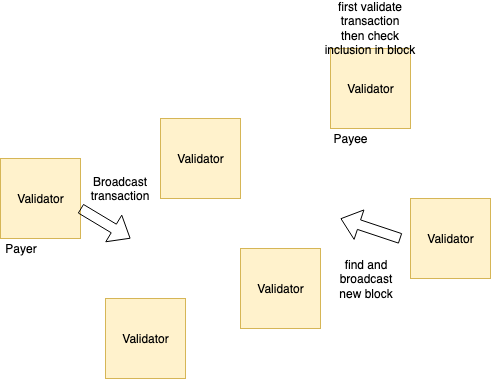
\includegraphics[width=\linewidth]{fig/NoLeader}
	\caption{Block creation with PoW}
	\label{fig:leader}
\end{figure}

This design give the following properties:
\begin{description}
	\item[Censorship] An adversary cannot prevent a node, it does not control from including a certain transaction.
	\item[Failures] Failure of individual nodes will not prevent the system from running.
	\item[Frequency] A high PoW difficulty ensures that blocks cannot be created faster than they can be distributed to members in the network.
	\item[Conflicting blocks] For a single entity to create two different blocks requires to solve PoW twice. This makes it difficult to publish two conflicting blocks.
	A high difficulty decreases the probability that two blocks are found concurrently.
\end{description}

\subsection{Adjustable difficulty}
Back in 2010 it was possible to join Bitcoin and create a new block using a simple desktop computer. Today specialized hardware (ASICs) is used to solve the PoW.
\begin{idea} To adjust to nodes joining and leaving the system, and nodes using different infrastructure (i.e. hardware) it is possible to adjust the hardness of the blockchain.
\end{idea}

\begin{definition}
Additional to the merkle root and nonce Bitcoin includes a timestamp in the	block (and in the PoW). This allows to compute the average time between two blocks every 2016 blocks and adjust the difficulty.
\end{definition}

\begin{note} on timestamps in a PoW blockchain
	
\begin{itemize}
	\item The time between blocks can vary significantly but this variance has little effect on the average time, taken over 2016 blocks.
	\item The timestamp can be set by the nodes when creating the block. When validating the block nodes check that the new block has a timestamp within 2 hours of their local clock.
\end{itemize}
\end{note}

\begin{lem}
	If we assume that the probability that the nodes find a new block within time $\Delta$ is constant and independent, and assume that the mean time to block creation is 10 minutes, we can compute the probability, that a block is created within $t$ seconds as
	\[
		P[\text{block created within } t \text{ seconds}] = 1- \left(\frac{599}{600} \right)^t
	\]
	\[
		P[\text{no block created within } t \text{ seconds}] = \left(\frac{599}{600} \right)^t
	\]
\end{lem}
\begin{proof}
Let $p$ be the probability that a block is found within 1 second.
Let $T$ be the random variable describing after how many seconds a new block is found. Since finding a block in a specific second is independent we get:
\[
P[T=t] = (1-p)^{t-1}p
\]
From Theorem~\ref{thm:bernoullitrials} it follows that $E[T] = \frac{1}{p}$.
If we assume $E[T]= 10 \text{min} = 600$ we get $p=\frac{1}{600}$.
\end{proof}

\begin{lem}
	Assume the current average block interval is $\Delta_1$. To adjust the average block interval to $\Delta_2$, we need to adjust difficulty from $d_1$ to
	\[
	d_2 := \frac{\Delta_1}{\Delta_2}\cdot d_1
	\]
	
\end{lem}

\begin{example}
	If the measured average delay or the last blocks is $5$ minutes and the desired delay is $10$ minutes you have to make PoW more difficulty (2 times). This is done by decreasing the target value $d$ by $0.5$.
	\[
		d_2 := \frac{d_1}{2}
	\]
	
\end{example}

\begin{example}
	If the measured average delay or the last blocks is $6$ minutes and the desired delay is $10$ minutes you have to adjust difficulty by
	\[
		d_2 := \frac{6}{10}d_1
	\]
	
\end{example}

\question{What is the probability that a block is found in:
\begin{itemize}
	\item Less than 3 minutes?
	\item Less than 1 minute?
	\item Less than 10 minutes?
	\item More than 15 minutes?
	\item More than 30 minutes?
\end{itemize}
Why is the probability for less than 10 minutes not 0.5?
}


\subsection{Fees and mining rewards}
Fees and mining rewards give an incentive to solve the PoW function.

\begin{definition}
When the sum of outputs of a transaction is larger than the sum of inputs, the difference is called \emph{fee}.	
\end{definition}

\begin{definition}
Every block in bitcoin contains a \emph{coinbase transaction}. This transaction has no input and a single output. The output value is the sum of a fixed reward (\emph{mining reward}) and the sum of all fees of transactions included in the block.
\end{definition}

\begin{note} There are different \textbf{pro's and con's for fixed rewards and fees:}
	\begin{itemize}
		\item In bitcoin the mining reward is halved every 4 years. Thus, only a finite amount of bitcoin will ever be created.
		\item The mining reward allows cheap transactions, since fees do not need to cover full mining expenses.
		\item Some research suggests, that if mining rewards are small compared to fees, mining becomes unstable.\footnote{\url{https://freedom-to-tinker.com/2016/10/21/bitcoin-is-unstable-without-the-block-reward/}}
		\begin{itemize}
			\item Miners may fight over transactions with big fees.
		\end{itemize}
		\item Mining awards are necessary to get money into circulation.
		\item Currently in bitcoin mining rewards are 12.5 bitcoin, while fees per block are less than 1 bitcoin.
	\end{itemize}
\end{note}

\question{How to determine fees? Banks/credit cards often take percentages.}

\begin{note} \textbf{How big should the fee be?}
Fees are determined by market economics, i.e. nodes choose which transactions to include. Usually those with highest fee.
	
Processing of transactions requires nodes to use network and processing capacities (for relaying and validating transactions). These expenses depend on the size of a transaction, but not on the value transferred. Therefore:
\begin{itemize}
	\item Fees in bitcoin are usually independent of the value of a transaction. Instead they depend on the size (in bytes) of the transaction.
\end{itemize}
\end{note}

\subsection{Forks and longest chain rule}
As mentioned above, PoW can reduce the probability for conflicting blocks to be proposed, but cannot prevent this from happening.

\begin{definition} A \emph{fork} in a blockchain is when multiple blocks are proposed with the same predecessor. Note that every block in a fork may be extended to a different chain.
\end{definition}

A fork is problematic since the different blocks or chains represent two versions of the world. 
	
\emph{Imagine your bank being undecided, wether you did or did not payed your rent.}

\begin{definition} (Longest chain rule) If a fork exists all nodes should adopt the longest chain.
\end{definition}

\begin{note} While the Longest chain rule is implemented in the standard bitcoin release, it is not enforced. It is possible to extend a different chain than the given by the longest chain rule. Doing this may change what is the longest chain. 
\end{note}

\begin{lem}
	Given two chains $c_1$ and $c_2$. To find a new block extending $c_1$ is equally likely as finding a new block extending $c_2$. This even holds, if nodes already spend significant resources to find a block extending $c_1$.
\end{lem}
\begin{proof} This follows from Lemma~\ref{lem:independent}.
\end{proof}

\begin{lem}
Assume two chains $c_1$ and $c_2$ where $c_1$ is longer than $c_2$. Further assume that most nodes follow the longest chain rule, trying to extend the longest chain.
	A new block is more likely to be eventually part of the longest chain, if it is added to $c_1$ rather than $c_2$.
\end{lem}
\begin{proof}
Chain $c_1$ is already longer than $c_2$. A new block would make $c_1$ even longer, while it would make $c_2$ at most equally long to $c_1$.
\end{proof}

\begin{figure}
	
	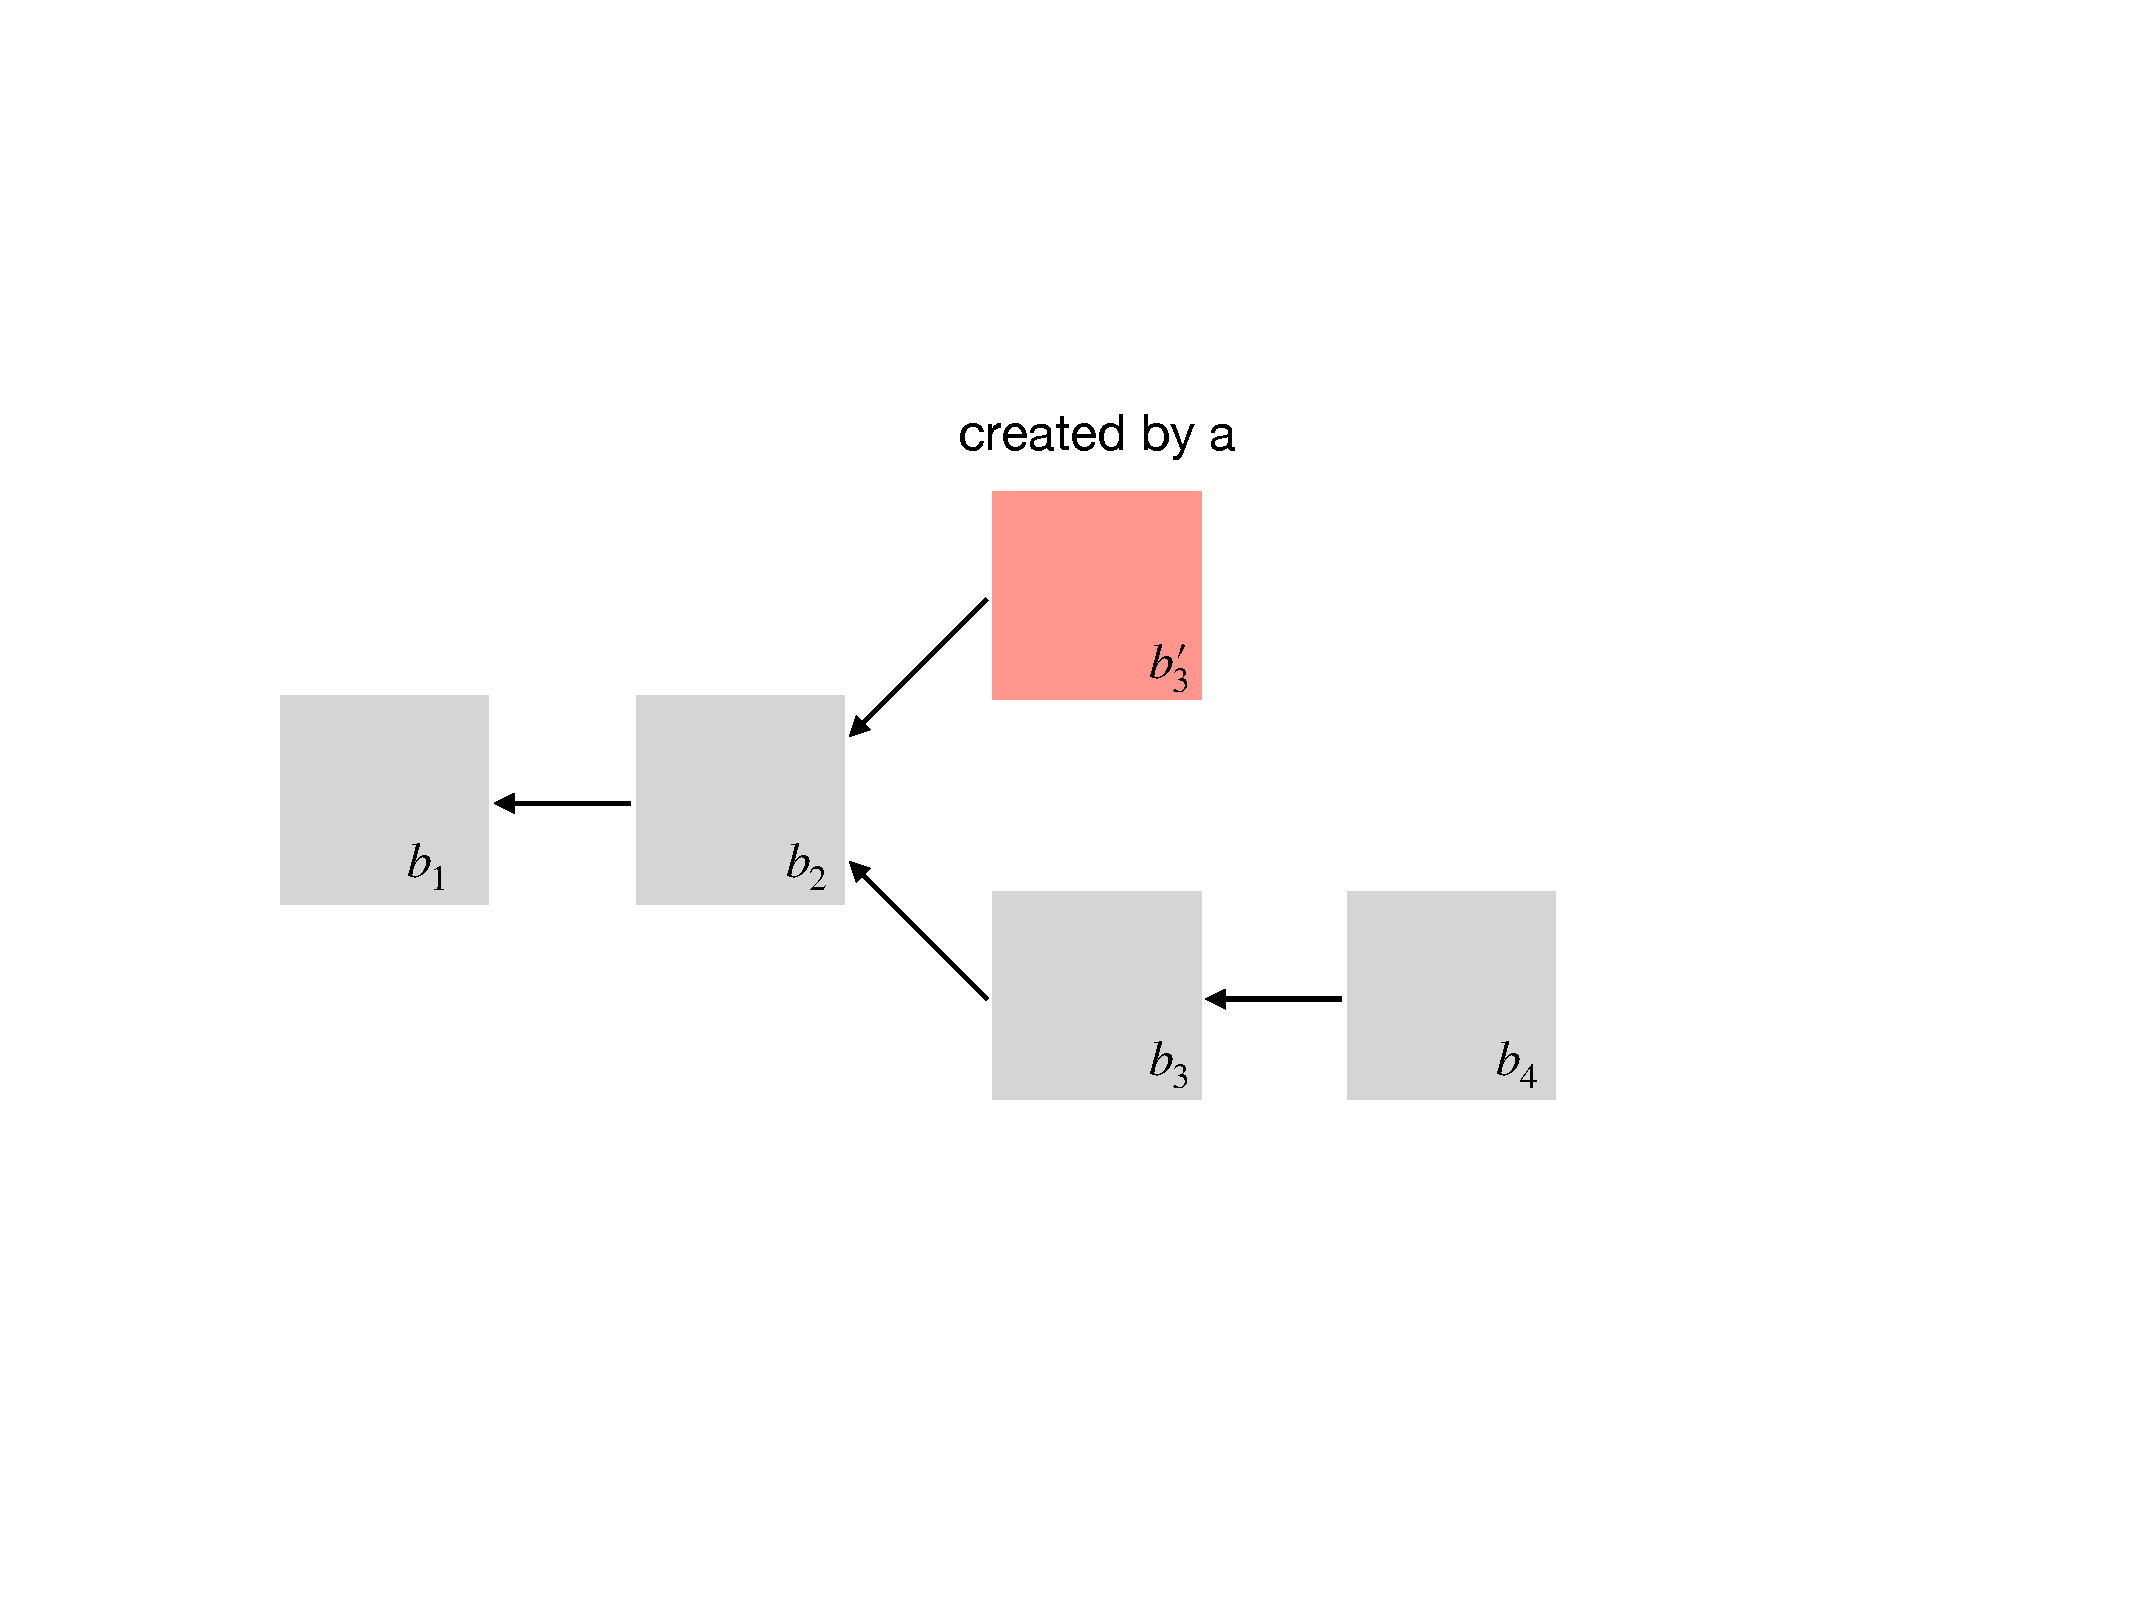
\includegraphics[width=\textwidth]{fig/fork}
	\caption{A fork in the blockchain. Two blocks extending $b_2$ where found.}
	\label{fig:fork}
\end{figure}

\begin{example}
	Figure~\ref{fig:fork} shows a fork. Two processes trying to extend block $b_2$ found a new block, $b_3$ and $b_3'$.
	
	Later another block $b_4$ was found, that extends $b_3$.
	According to the longest chain rule, all nodes will adopt the blocks $b_3$ and $b_4$ and discard the block $b_3'$.
	
	\textbf{Transactions that where only included in $b_3'$ but not in $b_3$ will not be part of the longest chain. They are effectively discarded.}
	\begin{description}
		\item[Coinbase transaction] The coinbase transaction in $b_3'$ is discarded. Thus the node that created $b_3'$ loses his block reward.
		\item[Double spending] Assume transactions $t$ and $t'$ spend the same output. Assume transaction $t'$ is included in $b_3'$ and $t$ is included in $b_3$. $t'$ is discarded together with $b_3'$. Since $b_3$ includes $t$, $t'$ cannot be included in a later block either.
	\end{description}
	
	 
\end{example}

\section{PoW and network latency}
\label{sec:fork}

We now analyze the probability that a fork occurs based on the network delay, i.e. the time it takes to broadcast a block to the different nodes.
Results in this section are taken from \href{https://www.gsd.inesc-id.pt/~ler/docencia/rcs1314/papers/P2P2013_041.pdf}{Decker and Wattenhofer, 2013.}

\begin{definition}
	We write $\delta$ for the average time it takes for a block until it is validated by a specific node in the network.
\end{definition}

\begin{note} Based on empirical evaluations, in the current bitcoin network, $\delta=12.6$ seconds. 
\end{note}

In the following theorem we assume that nodes have the same mining power and are following the longest chain rule.
\begin{theorem}
	\label{thm:fork}
	Let $p$ be the probability that a block is found within one second.
	Then the probability for a fork is
	\[
		1-(1-p)^\delta
	\]
\end{theorem}
\begin{proof}
The probability for a fork is the probability that the while the block is propagated, another block is found.
Thus $$P[\text{fork}] = 1- P[\text{no block found during dissemination}]$$

$$P[\text{no block found during dissemination}] = (1-p)^\delta$$
\end{proof}

\begin{cor}
\label{cor:longfork}
Let $P[\textnormal{fork}^l]$ be the probability that after a fork, both chains are extended by $l$ blocks. It holds
	\[
		P[\textnormal{fork}^l] \leq \left(1-(1-p)^\delta\right)^l
	\]
	
\end{cor}
\begin{proof}
Assume one chain $c_1$ is extended by one block. If a fork of this chain, $c_2$ is also extended, this has to happen before the new block on $c_1$ is propagated. Thus the probability that two chains in a fork are extended, is equal to the probability that a block on the second fork is found, while the block on the first fork is disseminated. This is less than the probability of a fork.
\end{proof}

Corollary~\ref{cor:longfork} says that the probability that a block is discarded because of a fork drops exponentially, with the numbers of blocks that are added after this block.

\begin{definition} We say that a transaction is \emph{confirmed}, if it is included in a block, and several blocks are added after this block.
	
In bitcoin, it is recommended to wait for additional 5 blocks, after the block including a transaction.	
\end{definition}

\question{
\begin{itemize}
	\item What is the probability for a fork in bitcoin?
	\item What is the probability that a fork extends for two blocks?
	\item What is the fork probability if the average network delay $\delta$ is 1 minute?
	\item What is the fork probability if the average block delay is 1 minute or 10 seconds?
\end{itemize}
}
	